
\section{Install}


\label{sec:installation}
	This section of the manual focuses on how to install the necessary dependencies and programs needed to run Bertini\_real on a user's computer. The instructions provided describe the process for Linux, Mac, and Windows operating systems. If you want to try to port Bertini\_real to another operating system, please contact Daniel Brake. 

	When installing Bertini\_real, there are a number of steps required in order to successfully install and run the program. They are:
\begin{enumerate}
\item Installing the \glspl{dependent}
\item Installing Bertini
\item Installing Bertini\_real
\end{enumerate}




\subsection{Dependencies}

Before installing Bertini and Bertini\_real, there are a number of packages that need to be installed. The method used to install these \glspl{dependent} changes depending on the operating system, so please be sure to read the section that describes your particular system.
The dependencies are: 
\begin{itemize}
\item a C++ compiler capable of the C++ 11 standard
\item an \gls{mpi} (such as MPICH2)
\item Boost $>$= 1.53
\item \gls{mpfr}
\item \gls{gmp}
\end{itemize} \cite[p.~4]{Br15}

	\subsubsection*{MATLAB}
The program MATLAB also needs to be installed on your computer as well. Instructions on how to install the program are not provided here. However, if you are associated with a university, or a research facility, they probably have download instructions on their technology support website (e.g. Notre Dame's OIT website). 

\subsubsection*{In Windows}

After installing MATLAB, please be sure to add \texttt{C:\textbackslash{User}\textbackslash{username}\textbackslash{\ldots}\textbackslash{matlab.exe}} to your PATH variable. 


\subsubsection*{In Unix \ GNU Linux}

If you do not already have MATLAB on the PATH, type \texttt{touch .bash\_profile}, which will create \texttt{.bash\_profile}, and then add \texttt{export PATH=/PATH/TO/MATLAB.app/bin:\$PATH}. This should result in the MATLAB executable being added to the path whenever opening terminal. 

If you are a Windows user, the instructions on had to add MATLAB to the \gls{path} are included in the Windows Instructions section


	\subsection{Instructions for GNU/Linux}

Use the package manager provided, such as apt-get, to install the dependencies into your preferred directory.

	\subsection{Instructions for OSX}

  \subsubsection{Preliminary Work}
  \begin{itemize}
    \item Download XCode 8 from the App Store to access its software development tools
    \begin{enumerate}
      \item In terminal, type `'xcode - select -- install`' (open XCode first before doing this)
    \end{enumerate}  
    \item It is recommended that Mac users install the program \href{http://brew.sh}{Homebrew} to use to install these packages. Once that has been done, installing the previously listed dependencies becomes simple. In terminal,  type \texttt{brew search \_\_\_\_} to list packages related to \_\_\_\_, where \_\_\_\_ is your search (for example, GMP, Boost, or MPICH2). To download via Homebrew, type in terminal \texttt{brew install \_\_\_\_}
     \begin{enumerate}
      \item Run it in the terminal
      \item Use directions from website on how to install it
      \item Authenticate it
     \end{enumerate}  
     \item Matlab: make sure to have it installed
  \end{itemize}

  \subsubsection{Installation}
  \begin{itemize}
    \item Install Bertini 1.5.1 (or latest version) from source
     \begin{enumerate}
      \item Make sure to download the source tarball (.tar.gz) from \href{http://bertini.nd.edu}{Bertini}
      \item Unpack the tarball (Double Click)
      \item Now use homebrew to install dependencies for Bertini1 (`brew install autoconf automake libtool mpfr gmp boost mpich`)
      \item In the terminal, move to the unpacked tarball for Bertini1
      \item `./configure`
      \item `make -j 4 \&\& make install`
    \end{enumerate}
    \item Get the source code for Bertinireal  
     \begin{enumerate}
      \item `which git`  if it's emtpy, then `brew install git`
      \item `mkdir code \&\& cd code`
      \item `git clone git://github.com/ofloveandhate/bertini\_real`
      \item `cd bertini\_real`
      \item `autoreconf -i`
      \item `./configure`
      \item `make -j 4 \&\& make install` 
     \end{enumerate} 
  \end{itemize}  


	\subsection{Instructions for Windows}
Unlike Linux or Mac computers, Windows users have additional pre-requisites that they need to install in order to use Bertini and Bertini\_real- they need to first install the program Cygwin.  Alternatively, with Windows 10 and Bash support upcoming, consider using Chocolatey or bash itself.

	\subsubsection{Cygwin}
Cygwin is a Linux- like environment for Windows. The other two operating systems that were discussed above were developed with Linux, while Windows was not. So, in order to run applications like Bertini that need Linux, there needs to be a program or environment that provides Linux for the applications that need it. 

	\paragraph*{How to Install Cygwin}

Cygwin can be found at \href{https://cygwin.com/install.html}{cygwin.com}. Please make sure to choose the version (either 32-bit or 64-bit) that is appropriate for your laptop. After the setup-x86.exe (or setup-x86\_64.exe) have downloaded, run the application, and follow the instructions.

\begin{longtabu} to \textwidth {
    X[1,c]
    X[1,c]}
\hline
\rowfont\bfseries
\textbf{Instructions} & \textbf{Screen Shot} \\
\hline  \\
\endfirsthead
\caption[]{\textit{Continued from previous page}}\\
\hline
\textbf{Instructions} & \textbf{Screen Shot} \\
\hline \\
\endhead
\bottomrule \multicolumn{2}{r}{\textit{Continued on next page}} \\
\endfoot
\bottomrule \multicolumn{2}{r}{\textit{Cite Source Here}} \\
\endlastfoot
Click `next' on the first screen. & 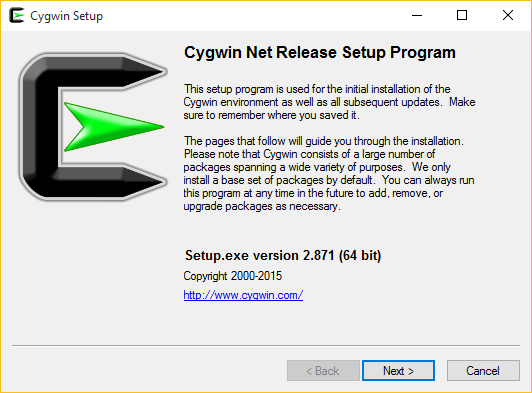
\includegraphics[width=0.4\textwidth]{CygwinInstall1}  \\  \\  \\ 
Select the `Install from Internet' option; click `next'. & 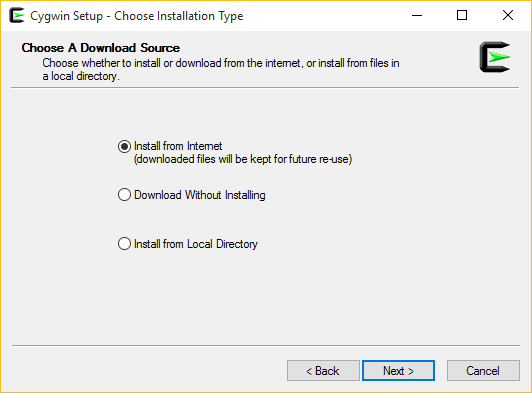
\includegraphics[width=0.4\textwidth]{CygwinInstall2}  \\  \\  \\ 
Enter the preferred installation directory; click `next'. & 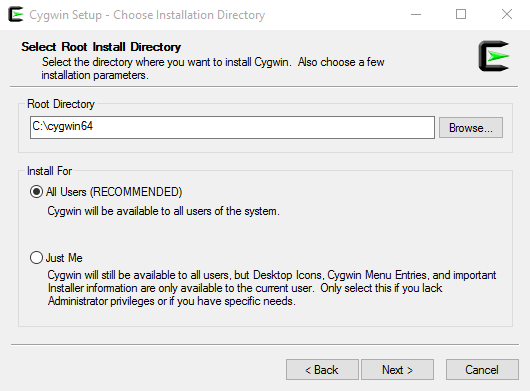
\includegraphics[width=0.4\textwidth]{CygwinInstall3}  \\  \\  \\ 
Choose a temporary installation folder; click `next'. & 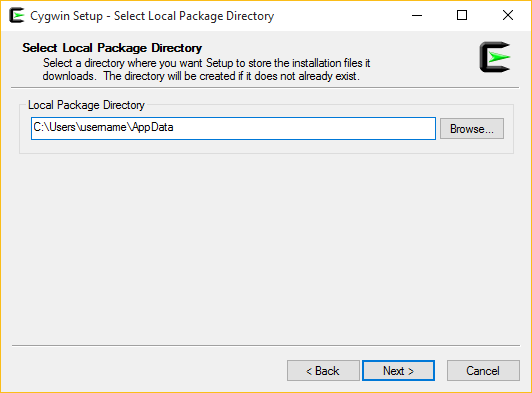
\includegraphics[width=0.4\textwidth]{CygwinInstall4}  \\  \\  \\ 
Select the `Direct Connection' option; click `next'. & 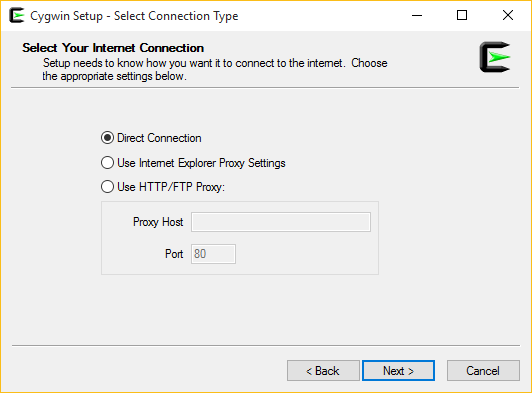
\includegraphics[width=0.4\textwidth]{CygwinInstall5}  \\  \\  \\ 
Choose a download site; click `next'. & 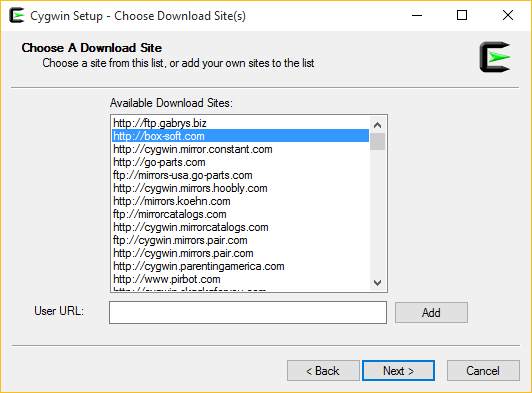
\includegraphics[width=0.4\textwidth]{CygwinInstall6} \\  \\  \\ 
Select the packages that you will need. , then click `next'. See below for more instructions & 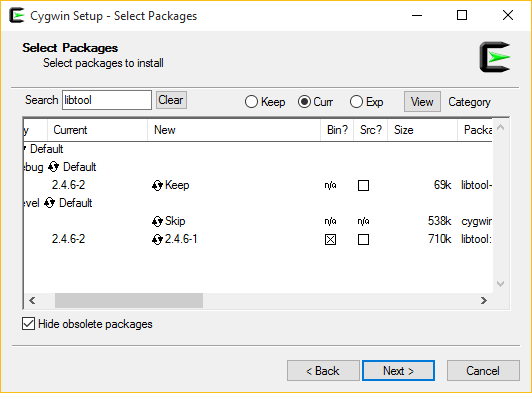
\includegraphics[width=0.4\textwidth]{CygwinInstall7}  \\  \\  \\ 
If during the course of installation, a message pops up and says that certain dependencies are required for the packages, click the `yes' button. When it has installed everything, select `finish'. &  \\  \\   
\end{longtabu}


		\subsubsection*{Selecting packages for Cygwin}
The list of packages that you will need for Bertini\_real can be found below. To find the packages, a user can type the name into the search in the top left of the menu,  which will then show the packages containing that name (e.g. `libtool'). To choose a package click on the text that says `Skip' until it changes to a version number (e.g. `2.4.6-1'). 

\begin{tabular}{ l l }
  autoconf & automake \\
  bash & bison \\
  boost (all the C and C++ libraries) & bzip2 \\
  X-11 & emacs (or nano or some other text editor that you prefer) \\
  flex & vim \\
  mingw-gcc-g++-4.7.3-1 & cygutils-X11 \\
  gmp & gcc \\
  mpc & mpfr \\
  libzip2 & xinit \\
   libtool & openmpi \\
  openssl& openssh \\
  tar & \\
\end{tabular}

	\subsection*{Setting up Cygwin}
		\subsubsection*{Initializing Paths}

In order to properly run Cygwin, you need to add Cygwin to the PATH variable. In order to do so, follow these steps:

\begin{enumerate}

\item Open the Control Panel and select `System'.

\item Select the `Advanced System Settings', and then the `Environment Variables' option. 

\item In the window that appears, select the system variable "PATH' and append \texttt{; C:\textbackslash{cygwin}\textbackslash {bin}} to the end of the PATH variable. When you are doing this, you can also append \texttt{; C:\textbackslash{path}\textbackslash{to}\textbackslash{matlab.exe}} to the end of the PATH as well.

\end{enumerate}

	\subsubsection*{Organizing Cygwin}

	Once Cygwin and MATLAB have been added to the PATH variable, you are now ready to open and run Cygwin. For users who are not familiar with Cygwin, a good reference sheet can be found \href{http://faculty.nps.edu/kmsquire/cs2900/cygwin/fwcygwinref.pdf}{here}.

As part of the installation process, Cygwin will automatically configure and install the packages you selected. This is useful, since it saves a lot of time for the user. However, this also allows a Cygwin user to go and be able to automatically use some of these applications, such as `libtoolize'. Libtoolize, one of the packages that was installed with \texttt{setup\-86x.exe} allows a user to set up a shared library format. In other words, a user doesn't have to call each different library; they are already set up and in the same place.

When I set up Cygwin, I created a new folder located in \texttt{\textbackslash{usr}\textbackslash{local}} that would contain any downloaded files from the Internet that would be used with Cygwin.\par

When setting up Cygwin, I found that in order to install the dependencies that are needed for Bertini and Bertini\_real, they had to be downloaded from the Internet. The following instructions describe how to install these dependencies and finish setting up Cygwin, and were paraphrased from \href{http://cygwin.wikia.com/wiki/How_to_install_GCC_4.3.0}{How to Install a Newer Version of GCC}.

	\subsubsection*{Installing Dependencies}
As stated earlier, the dependencies that need to be downloaded are: 

\begin{tabular}{ l r c }
  C++ compiler & gcc(Cygwin) & \checkmark \\
  MPI & openmpi(Cygwin) & \checkmark \\
  Boost & boost(Cygwin) & \checkmark \\
  \gls{gmp} & gmp(Cygwin) & \checkmark \\
  \gls{mpfr} & \href{http://www.mpfr.org/index.htm}{here} &  \\
  \gls{mpc} & \href{http://www.multiprecision.org}{here} &  \\
\end{tabular} 

Once you have downloaded the programs from the sites, put the zipped files in the folder that you created in \\ \texttt{\textbackslash{usr}\textbackslash{local}\textbackslash{your\_folder}}. Then, in Cygwin, enter \texttt{your\_folder}. 

	\subsubsection* {Linking Cygwin Environment Paths}
After logging into Cygwin, a user needs to set up their environment paths inside the terminal before they set up the files they downloaded. In order to see how the paths currently are set up, either type the following code into the terminal, or copy it and paste it into the terminal: 

\begin{center}\begin{minipage}{0.9\linewidth}

\begin{lstlisting}[language=c++, caption=Adapted from \cite{installnewerGCC}, captionpos=b]
   echo ;\
   echo LD_LIBRARY_PATH=${LD_LIBRARY_PATH}; \
   echo LIBRARY_PATH=${LIBRARY_PATH}; \
   echo CPATH=${CPATH}; \
   echo PATH=${PATH}; \
   echo   \cite{installnewerGCC}
\end{lstlisting}
\end{minipage}\end{center}

Some things to keep in mind while setting up the environment variables \gls{ldlib}, \gls{lib}, and \gls{cpath}:
\begin{itemize}
\item \textbf{LD\_LIBRARY\_PATH} and \textbf{LIBRARY\_PATH} should contain /usr/local/lib (\textbf{LIBRARY\_PATH} shall not be set on Enterprise Linux Enterprise Linux Server release 5.5 (cartage)) 
\item \textbf{CPATH} should contain /usr/local/include
\item If \textbf{PATH} contains \texttt{c:/windows/system32} (or \texttt{/cygdrive/c/windows/system32}; case-insensitive), it should be after /bin and /usr/bin. Otherwise the scripts will try to run Windows sort.exe instead of the Unix command with the same name.
\end{itemize}

To change or modify the different variables, you can use the code below (or you can change the variables in the Control Panel, as shown earlier): 
\begin{center}\begin{minipage}{0.9\linewidth}

\begin{lstlisting}[language=c++, caption=Adapted from \cite{installnewerGCC}, captionpos=b]
   setenv LD_LIBRARY_PATH /usr/local/lib
   setenv LIBRARY_PATH /usr/local/lib
   setenv CPATH /usr/local/include
\end{lstlisting}
\end{minipage}\end{center}

However, if Cygwin shows a message such as \texttt{-bash: setenv: command not found}, then you need to use the code below: 
\begin{center}\begin{minipage}{0.9\linewidth}

\begin{lstlisting}[language=c++, caption=Adapted from \cite{installnewerGCC}, captionpos=b]
   export LD_LIBRARY_PATH=/usr/local/lib
# Depending on system, LIBRARY_PATH shall not be set - 
#  export LIBRARY_PATH=
   export LIBRARY_PATH=/usr/local/lib
   export CPATH=/usr/local/include
\end{lstlisting}
\end{minipage}\end{center}

	\subsubsection*{Building and Installing Packages}
Now that the environment variables are set up, we can now build and set these packages. 

Perform the following build/install steps for the \textbf{MPFR} and \textbf{MPC} packages \textit{\underline{in that order}}:

\begin{enumerate}

\item cd to your workspace directory (above, e.g., cd \textbf{\texttt{\textbackslash{usr} \textbackslash{local} \textbackslash{your\_folder}}})
\item Extract the tarball using tar (e.g., \textbf{\texttt{tar -xf mpfr-3.1.3.tar.bz2}}). This will create a sub-folder with the source for the given package
cd into that source folder (e.g., \textbf{\texttt{cd mpfr-3.1.3}})
\item Type \textbf{\texttt{libtoolize}} into the command line and press enter. This will add the files, once they have been compiled, to the shared library.
\item Generate {\tt configure}, by running the command {\tt autoreconf -i}.
\item Read the README and/or INSTALL file if present
\item Note that for the current version of \textbf{mpc (0.9)} there is a change that may need to be made to have the build work successfully. You need to edit the line of "mpc.h"

\begin{minipage}{0.9\linewidth}
\centering
    \begingroup
    \texttt{%
    \#if defined(\_\_MPC\_WITHIN\_MPC) \&\& \_\_GMP\_LIBGMP\_DLL}
    to
    \texttt{%
    \#if defined \_\_GMP\_LIBGMP\_DLL}
    \endgroup
\end{minipage}

\item run \textbf{\texttt{./configure}} (this will check the configuration of your system for the purpose of this package)(you also need specify \textbf{\texttt{--enable-static --disable-shared}} when compiling the library)
\item run \textbf{\texttt{make}} (this will build the package; \textbf{\texttt{-j}} can speed things up here)
\item run \textbf{\texttt{make check}} (strongly recommended but optional; this will check that everything is correct)
\item run \textbf{\texttt{make install}} (this will install all the relevant files to the relevant directories)
\item run \textbf{\texttt{make clean}} (optional; this will erase intermediate files - important if you are re-attempting a broken build!)

\end{enumerate}








\clearpage
	\subsection{Installing Bertini and Bertini\_real}

Once all of the dependencies have been installed, now Bertini and Bertini\_real can be installed. The zip file for Bertini can be found
\href{http://bertini.nd.edu/download.html}{here}, while the download site for Bertini\_real can be found
\href{http://www.bertinireal.com/download.html}{there}

Move these downloads to your terminal, and unzip and install the two programs. To unpack the directory, just run \texttt{tar -zxvf FILE\_NAME} into the command line while in the folder that the .tar.gz is located. (For Cygwin users, this means going through the same steps as you did for GMP, MPFR, and MPC.) Be sure to install Bertini \textit{\underline{before}} Bertini\_real!!


	\subsection{Setting up MATLAB}
After you have set up Bertini and Bertini\_real, you probably want to be able to see a 3D rendering of your solutions. In order to do so, go to the GitHub  \href{https://github.com/ofloveandhate/bertini_real/tree/master/matlab_codes}{Bertini\_real site} and download the .zip file. I recommend that a new folder is created and that the zip folder goes inside this `master folder'. Unfortunately, the user also has to download each of the functions that are on the same level as the zip folder- e.g. \texttt{dehomogenize.m}, \texttt{find\_constant\_vars.m}, etc. and save those in the `master folder' as well. Make sure that this `master folder' is linked to the folder where the Bertini and Bertini\_real solutions will be located. Once all of these functions and the zip folder are downloaded and saved, then you will be able to successfully use MATLAB in conjunction with Bertini and Bertini\_real. 

\begin{centering}
Congratulations, you have now made it through the installation process. There are some additional features that can also be installed if you so desire, as well as a practice run in order to verify that everything installed correctly.
\end{centering}



		\subsubsection{Parallel Bertini\_real Installation}

Bertini\_real is parallel enabled, using MPI.  You cannot build Bertini\_real without support for MPI at the current time.   To use multiple processors to decompose a real object, call Bertini\_real as you would any other MPI program: \texttt{mpiexec [options] bertini\_real}.











\subsection{Testrun -- the Cayley Cubic}

Now that everything has been installed, we can now do a test run, to make sure that everything is working properly. To test this program, we will try to generate a Cayley Cubic using the above programs, following a number of steps. The first step is to create an input file. Open up a text editor in your terminal and create a file called \texttt{input}. 

Below is the text for this input file.. A key feature to notice is the second line, where the \texttt{tracktype} configuration is set to 1. This configuration setting is necessary for Bertini\_real to run. 

\begin{center}\begin{minipage}{0.9\linewidth}
\begin{lstlisting}[language=c++, caption={\tt input} for the Cayley Cubic, captionpos=b]
CONFIG 
tracktype:1;

END;
INPUT
variable_group x, y, z;
function f;
f = 4 * (x^2 + y^2 + z^2) + 16*x*y*z - 1;
END;
\end{lstlisting}
\end{minipage}\end{center}

Once the input file is created, we can now run Bertini. Simply navigate in the command line to the directory of the input file and type \texttt{bertini} or \texttt{bertini input}.  You may need to type in the entire pathway to where Bertini is located, if it's not in the same folder, so the command line read \newline \texttt{/cygdrive/path/to/BertiniSource\_v1.5/bertini-serial.exe input}\- \\ \textbf{Cygwin users:} A user may also use \texttt{bertini-serial.exe} (or \texttt{bertini\_parallel.exe}). This will run Bertini, creating the Numerical Irreducible Decomposition needed for Bertini\_real. The following should print to the terminal or shell:

\begin{center}\begin{minipage}{0.9\linewidth}
\centering
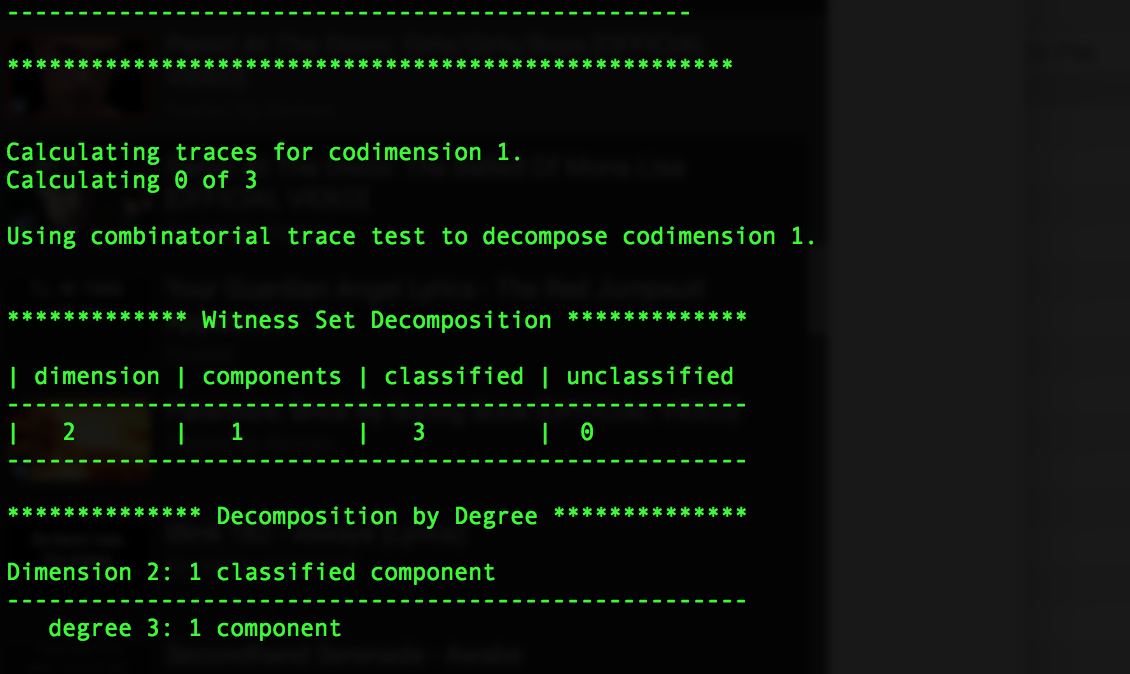
\includegraphics[width=0.6\textwidth]{CayleyCubicBertiniRun.png}
\end{minipage}\end{center}

Once Bertini is finished, the output can be verified as satisfactory (or not). Then, Bertini\_real can be run by calling \texttt{bertini\_real} in the command line. Cygwin users, the same rules that applied to Bertini also apply to Bertini\_real, so be sure to include that `.exe' at the end! However, if the input file used was named `input', no file name is needed at the end of the command line. This program should run for roughly 20-30 seconds, with the final terminal/shell output appearing below:

\begin{center}\begin{minipage}{0.9\linewidth}
\centering
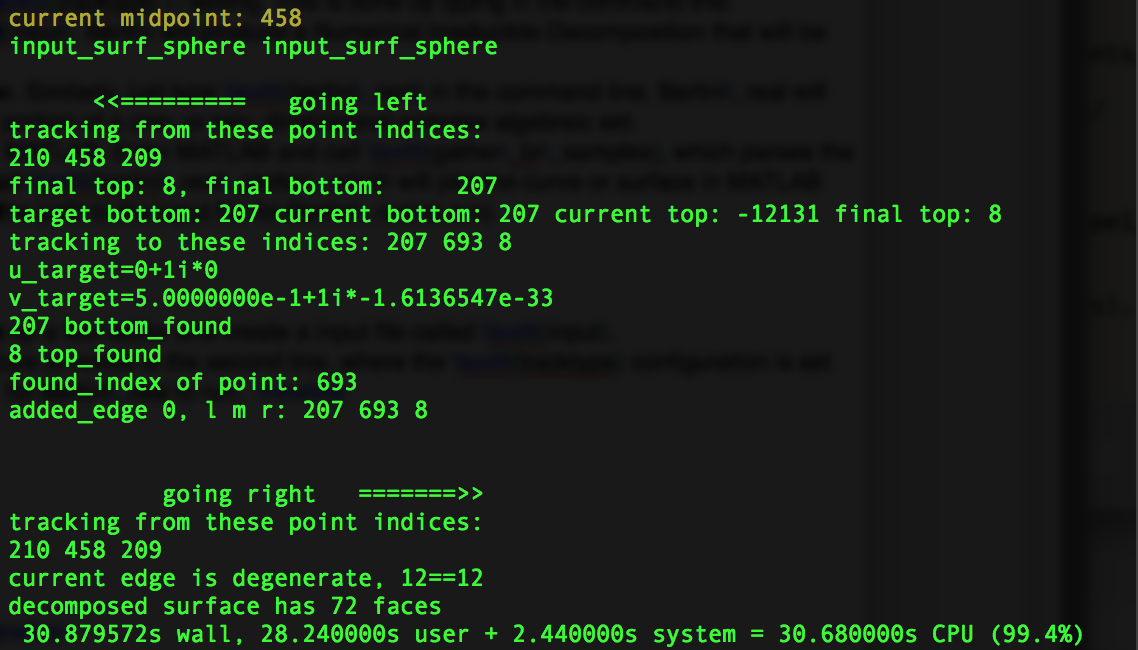
\includegraphics[width=0.6\textwidth]{CayleyCubicBertiniRealRun}
\end{minipage}\end{center}

Finally, MATLAB can be used to visualize the result from the Bertini\_real run. Open MATLAB and enter the `master file', which must be linked to the folder where the Bertini\_real solutions are located. This can be done by first making sure that you are currently in the `master folder', then typing \texttt{addpath(`C:\textbackslash{cygwin64}\textbackslash{path}\textbackslash{to}\textbackslash{solutions\_folder}')} into the command window and pressing enter. Then you can call \texttt{gather\_br\_samples} in the command window, which generates a .mat file. Then, call \texttt{bertini\_real\_plotter\-}. This will create a MATLAB figure, pictured below.

\begin{center}\begin{minipage}{0.9\linewidth}
\centering
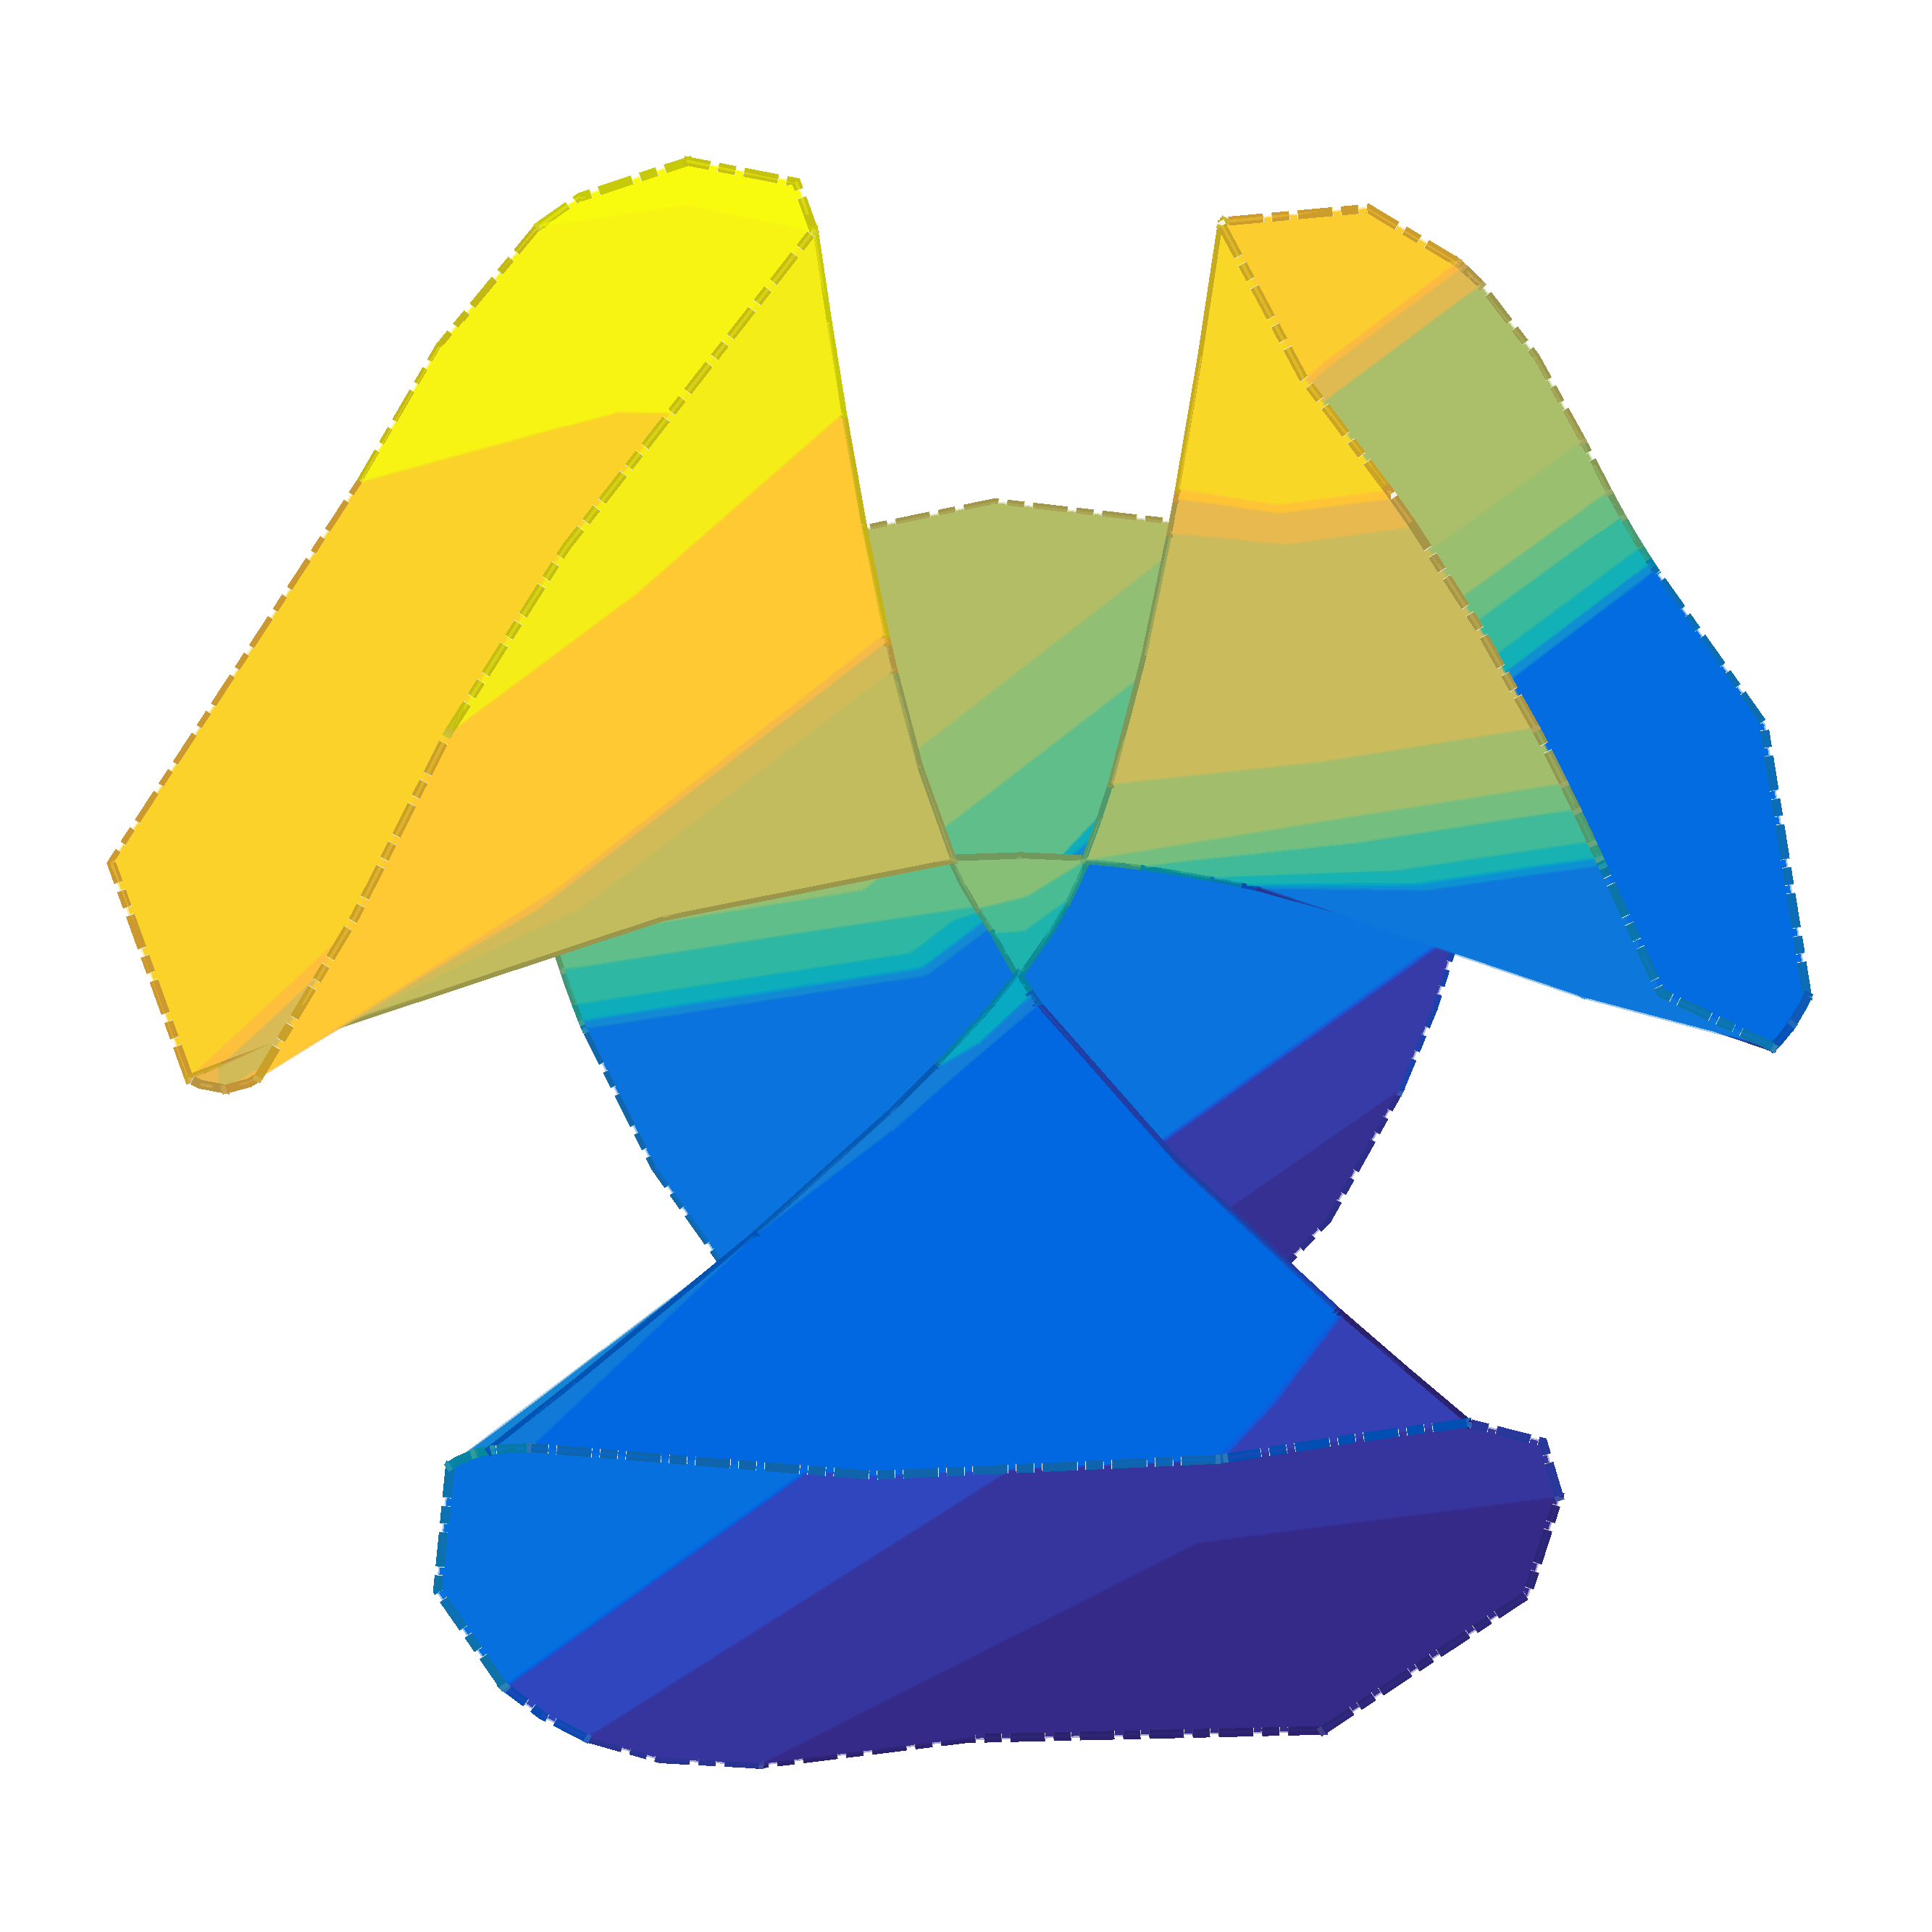
\includegraphics[width=0.6\textwidth]{CayleyCubic}
\end{minipage}\end{center}


If you've been able to reproduce the above figure, then you've mastered the basics of Bertini\_real. 





	\subsection{Other Operating Systems}
If you would like to use Bertini\_real on operating systems that haven't been listed in this manual, please contact Daniel Brake to discuss porting Bertini\_real to your system.


